\section{Эволюция звезд –- основные стадии.}

\subsection{Образование звезд}

Звёзды образуются из областей гравитационной неустойчивости в облаках межзвёздного газа. 

\paragraph{Масса Джинса}

Чтобы началось звездообразование, нужно, чтобы полная энергия была отрицательной, то есть, (по теореме вириала) если гравитационная энергия по модулю больше удвоенной кинетической.

Критическая масса, при которой \textit{может} начаться звездообразование называется массой Джинса.

\begin{equation*}
2 K + U = 0 \implies
 \begin{cases}
   K = N \frac{3}{2} k T\\
   U = - \frac{3}{5}\frac{GM^2}{R}
 \end{cases} \implies
 N k T = \frac{M}{m} k T = \frac{GM^2}{5R} = \frac{GM^2}{5}\left(\frac{4\pi\rho}{3 M}\right)^{1/3}
\end{equation*}

\begin{equation}
   \boxed{ M_j = \left(\frac{5 k T}{Gm} \right)^{3/2} \left(\frac{3}{4\pi\rho} \right)^{1/2}}
   \label{eq:9_jeans}
\end{equation}

Из формулы \ref{eq:9_jeans} видно, что звезды формируются из более \textbf{плотных} и \textbf{холодных} областей -- именно они начнут коллапсировать. 

Изначально сжимется большой фрагмент облака ($> 10^3 M_{sun}$) (поэтому часто звезды образуются \textit{скоплениями}). По мере сжатия растет плотность, но не температура (облако прозрачно для собственного излучения, которое уносит энергию), джинсовская масса падает и объект разделяется на более мелкие, имеющие звездные/субзвёздные массы. Есть причины полагать, что таким образом могут формироваться не только звезды, но и бурые карлики, и может быть планеты.

\paragraph{Первые звезды}

Таким образом формировались первые звезды (100 млн лет после Большого взрыва), так как состояли только из легких элементов. Газу было трудно остывать, потому что излучение провоцируют колебательные уровни молекул(типа C-O, которые в ранней Вселенной еще не сформировались). Таким звездам было трудно достичь низких джинсовых масс, так как единственная существовавшая колебательная молекула для них H-H. Они были большие, жили мало (1-2 млн лет) и быстро взрывались как сверхновые, распространяя тяжелые элементы 

\paragraph{Теорема вириала для звезд}

Звезды являются очень стабильными объектами, так как отвод тепла заставляет звезду сжиматься, а значит нагреваться, и наоборот, нагрев влечет за собой расширения и псоледующее остывание. Можно сказать, что звезды обладают ''отрицательной теплоемкостью'' или ''обратной связью''.

\newpage

\subsection{Популяции звезд}

Выделяют три типа популяции (населения) звезд:
\begin{figure}
    \centering
    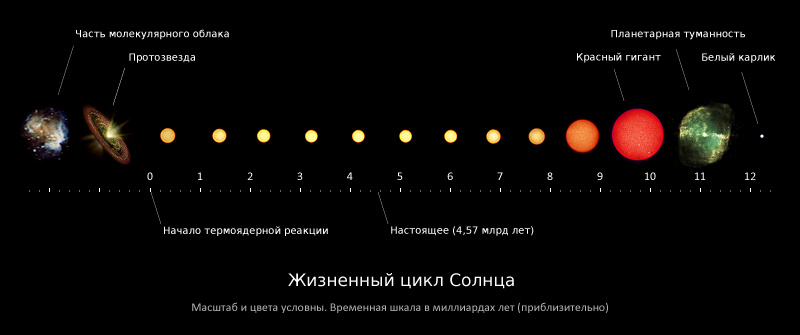
\includegraphics[width = 0.9\textwidth]{Pictures/9_Solar-evolution.png}
    \label{fig:9_solar}
\end{figure}

\begin{itemize}
    \item Популяция III -- самые первые звёзды.
    
    Состоят из водорода и гелия -- первичного газа Вселенной.
    \item Популяция II -- старые звёзды Галактики.
    
    \item Популяция I -- ''современные'' звёзды (до 10 млрд. лет назад).
    Особенность -- хим. состав (содержание тяжелых элементов).
    
\end{itemize}
\subsection{Эволюция звезд}

Классифицировать звезды удобно с помощью диаграммы \textbf{Герцшпрунга - Рассела}. 
\begin{wrapfigure}[18]{r}{0.63\linewidth}
  \centering
    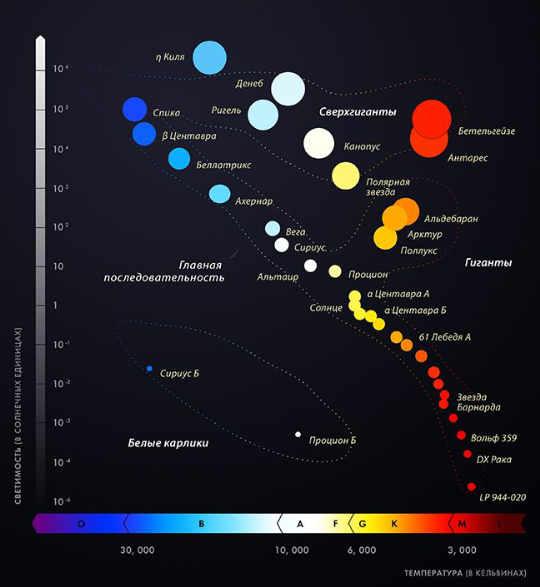
\includegraphics[width=0.65\linewidth]{Pictures/9_diag.png}
  \caption{Диаграмма Герцшпрунга-Рассела}
  \label{fig:9_diag}
\end{wrapfigure}Это зависимость светимости звезды от температуры (чем левее, тем горячее). В реальности не получалось точно измерять эти параметры,  поэтому по горизонтальной оси откладывали спектральные характеристики, а по вертикальной -- звездную величину для данного скопления. Оказалось, что подавляющее большинство звезд ложится на одну линию, которую назвали \textit{главная последовательность}. 90$\%$ жизни звезды проводят, находясь на главной последовательности, так как она соответствует стадии превращения водорода звезды в гелий.

\newpage

\begin{figure}[h]
\begin{minipage}[h]{0.49\linewidth}
\center{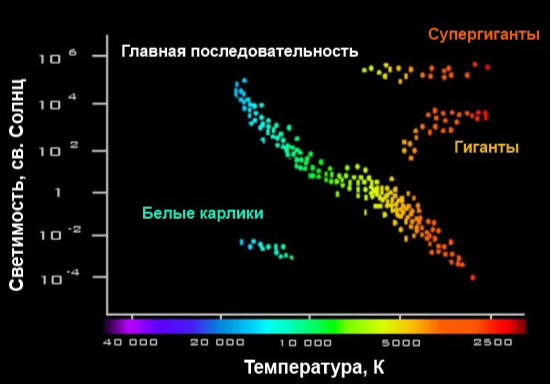
\includegraphics[width=0.9\linewidth]{Pictures/9_life.png} \\ а) Главная последовательность}
\end{minipage}
\hfill
\begin{minipage}[h]{0.49\linewidth}
\center{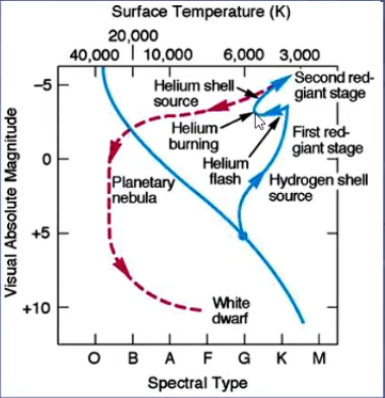
\includegraphics[width=0.6\linewidth]{Pictures/9_life2.png} \\ б) Эволюция Солнца}
\end{minipage}
\caption{Эволюция одиночной звезды.}
\label{fig:9_life}
\end{figure}

\begin{itemize}
    
    \item После того, как весь водород в ядре заканчивается, теряется источник энергии. Звезда остывает (теряет энергию), а значит, сжимается (становится более плотным), от этого нагревается. Этот процесс будет происходить, пока не появятся условия для начала термоядерного горения ядра. Не для всех звезд это возможно. 
    
    \item Из-за сжатия повышается температура и плотность на внешней границе ядра (вне ядра все еще есть водород). Если возникают условия для начала термоядерных реацкия \textit{вне} ядра, водород становится \textbf{слоевым источником} очень большой мощности. Резко растет светимость звезды, она расширяется и превращается в \textbf{красный гигант}.
    
    \item Ядро внутри сжимается. Если достигаются условия горения гелия в ядре, звезда уходит с ветки красных гигантов (рис. \ref{fig:9_life} (б) ), ее температура повышается при постоянной светимости.
    
    \item Гелий в ядре заканчивается (быстрее, чем водород, температуры выше). Образуется углеродно - кислородное ядро, наступает вторая стадия красного гиганта (\textbf{гигант - асимптотическая ветвь}).
    
    \item Ядро сжимается и пытается перейти на следующую стадию. У маломассивных звезд (типа Солнца) ядро начнет остывать, сбрасывать внешнюю оболочку, будет уменьшаться светимость и образуется \textbf{белый карлик}. В дальнейшем он будет остывать, переходя вправо по линии спектральных классов (горизонтальная ось рис. \ref{fig:9_life} (а) ).
    
    \item Если звезда достаточно массивная, в ядре начинается горение углерода и кислорода, звезда взрывается и превращается в нейтронную звезду или чёрную дыру.
    
\end{itemize}

\newpage

\subsection{Особенности треков для звезд разной массы}

\paragraph{Протозвезды} -- объекты высокой светимости (из-за того что она сжимается) и низкой температуры. Излучение преимущественно в инфракрасном диапазоне.

\paragraph{Массивные звезды} Для массивных здезд есть неопределенности, поэтому расчеты не согласуются между собой полностью, но общая черта заключается в значительно меньшем размере петли трека(рис. \ref{fig:9_life} (б) ), чем для звезд сравнимых по массе с Солнцем. 


    
\paragraph{Фанфакты} 

\begin{itemize}
    \item Чем меньше металличность звезды, тем раньше она образовалась.
    \item Возраст звезды на главное последовательности трудно определить.
    \item Основная характеристика звезды -- масса. Чем больше масса, тем больше звезда излучает и тем меньше живет.
    \item Время жизни звезд с массой меньше солнечной сравнимо с временем жизни галактики.
    \item \href{http://nuclphys.sinp.msu.ru/m_un/mun16.htm}{Полезная ссылочка}, а тут \href{https://habr.com/ru/post/366947/}{красивые картиночки}.
\end{itemize}
